\documentclass[12pt,a4paper]{article}

\usepackage[margin=1in]{geometry}
\usepackage{amsmath, amssymb, amsthm}
\usepackage{enumitem}
\usepackage{tikz}
\usetikzlibrary{arrows.meta, positioning}

\setlength{\parindent}{0pt}
\setlength{\parskip}{6pt}

\newtheoremstyle{notestyle}
  {8pt}
  {8pt}
  {\normalfont}
  {}
  {\bfseries}
  {.}
  {0.5em}
  {}

\theoremstyle{notestyle}
\newtheorem{definition}{Definition}
\newtheorem{example}{Example}
\newtheorem{theorem}{Theorem}

\newenvironment{answer}
{\par\textbf{Answer.}\ }
{\hfill$\square$\par}

\title{\textbf{Supplementary Practice: Irreducible Markov Chains}}
\author{MA4034: Time Series and Stochastic Processes}
\date{}

\begin{document}
\maketitle

\section{Main Idea}

\begin{definition}[Accessible]
State $j$ is accessible from state $i$, written
\[
i\to j,
\]
if there exists some $n\geq 0$ such that
\[
p_{ij}^{(n)}>0.
\]
This means that there is a positive-probability path from $i$ to $j$.
\end{definition}

\begin{definition}[Communicating States]
States $i$ and $j$ communicate, written
\[
i\leftrightarrow j,
\]
if
\[
i\to j
\qquad\text{and}\qquad
j\to i.
\]
\end{definition}

\begin{definition}[Irreducible Markov Chain]
A Markov chain is \textbf{irreducible} if every pair of states communicates. That is, for every $i,j\in S$,
\[
i\leftrightarrow j.
\]
\end{definition}

\textbf{Simple test.} A Markov chain is irreducible if the transition diagram is one connected communicating system: from any state, we can eventually reach every other state.

\section{Theorem: Three Possibilities for an Irreducible Chain}

\begin{theorem}
For an irreducible Markov chain, there are three possibilities:
\begin{itemize}[leftmargin=1.2cm]
    \item all states are positive recurrent,
    \item all states are null recurrent,
    \item all states are transient.
\end{itemize}
\end{theorem}

This theorem says that in an irreducible chain, all states have the same recurrence type. We cannot have one state positive recurrent and another state transient in the same irreducible chain.

\[
\boxed{\text{Irreducible chain} \Rightarrow \text{classify the whole chain, not states separately.}}
\]

\subsection{Case 1: All States Positive Recurrent}

A finite irreducible Markov chain is always positive recurrent. For example:

\begin{center}
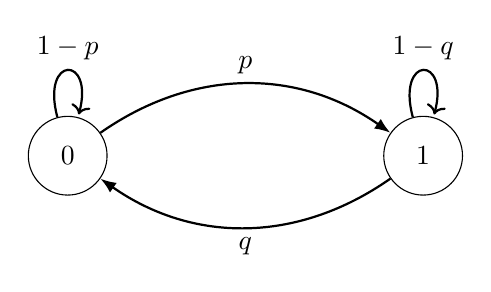
\begin{tikzpicture}[
  state/.style={circle, draw, minimum size=10mm},
  edge/.style={-{Latex[length=2mm]}, thick},
  bend angle=35
]
\node[state] (0) {$0$};
\node[state, right=35mm of 0] (1) {$1$};

\draw[edge] (0) edge[bend left] node[above] {$p$} (1);
\draw[edge] (1) edge[bend left] node[below] {$q$} (0);
\draw[edge] (0) edge[loop above] node {$1-p$} (0);
\draw[edge] (1) edge[loop above] node {$1-q$} (1);
\end{tikzpicture}
\end{center}

Here assume
\[
0<p<1,\qquad 0<q<1.
\]

Then state $0$ can reach state $1$, and state $1$ can reach state $0$. Hence the chain is irreducible.

Since the state space is finite,
\[
S=\{0,1\},
\]
both states are positive recurrent.

\[
\boxed{\text{All states are positive recurrent.}}
\]

\textbf{Meaning.} The chain returns to each state with probability 1, and the expected return time is finite.

\subsection{Case 2: All States Null Recurrent}

An infinite irreducible chain may be recurrent but not positive recurrent. In that case, all states are null recurrent.

A standard example is the fair gambler's chain:

\begin{center}
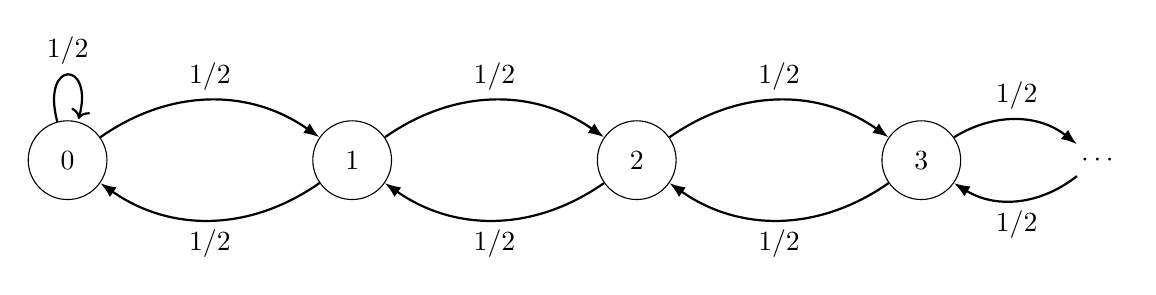
\begin{tikzpicture}[
  state/.style={circle, draw, minimum size=10mm},
  edge/.style={-{Latex[length=2mm]}, thick},
  bend angle=35
]
\node[state] (0) {$0$};
\node[state, right=26mm of 0] (1) {$1$};
\node[state, right=26mm of 1] (2) {$2$};
\node[state, right=26mm of 2] (3) {$3$};
\node[right=14mm of 3] (dots) {$\cdots$};

\draw[edge] (0) edge[loop above] node {$1/2$} (0);
\draw[edge] (0) edge[bend left] node[above] {$1/2$} (1);
\draw[edge] (1) edge[bend left] node[below] {$1/2$} (0);
\draw[edge] (1) edge[bend left] node[above] {$1/2$} (2);
\draw[edge] (2) edge[bend left] node[below] {$1/2$} (1);
\draw[edge] (2) edge[bend left] node[above] {$1/2$} (3);
\draw[edge] (3) edge[bend left] node[below] {$1/2$} (2);
\draw[edge] (3) edge[bend left] node[above] {$1/2$} (dots);
\draw[edge] (dots) edge[bend left] node[below] {$1/2$} (3);
\end{tikzpicture}
\end{center}

The state space is
\[
S=\{0,1,2,\ldots\}.
\]

From any state, we can move down step by step to state $0$, and from state $0$ we can move up step by step to any other state. Therefore the chain is irreducible.

For this fair case, the chain returns to states with probability 1, but the expected return time is infinite. So the states are null recurrent.

\[
\boxed{\text{All states are null recurrent.}}
\]

\textbf{Meaning.} The chain returns eventually with probability 1, but the average waiting time for return is infinite.

\subsection{Case 3: All States Transient}

An infinite irreducible chain can also be transient. A typical example is a biased gambler's chain with upward drift:

\begin{center}
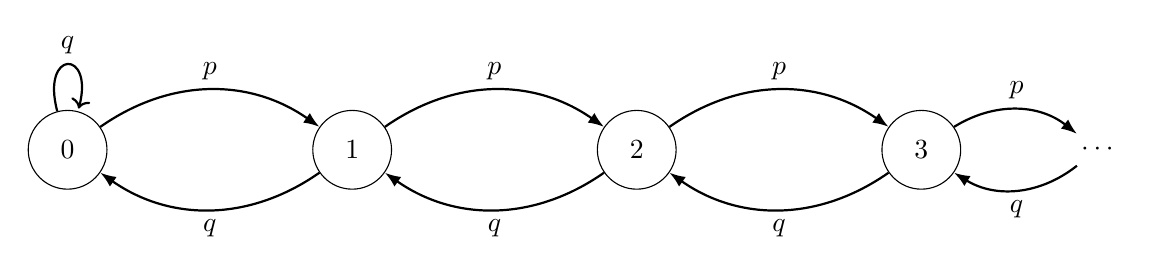
\begin{tikzpicture}[
  state/.style={circle, draw, minimum size=10mm},
  edge/.style={-{Latex[length=2mm]}, thick},
  bend angle=35
]
\node[state] (0) {$0$};
\node[state, right=26mm of 0] (1) {$1$};
\node[state, right=26mm of 1] (2) {$2$};
\node[state, right=26mm of 2] (3) {$3$};
\node[right=14mm of 3] (dots) {$\cdots$};

\draw[edge] (0) edge[loop above] node {$q$} (0);
\draw[edge] (0) edge[bend left] node[above] {$p$} (1);
\draw[edge] (1) edge[bend left] node[below] {$q$} (0);
\draw[edge] (1) edge[bend left] node[above] {$p$} (2);
\draw[edge] (2) edge[bend left] node[below] {$q$} (1);
\draw[edge] (2) edge[bend left] node[above] {$p$} (3);
\draw[edge] (3) edge[bend left] node[below] {$q$} (2);
\draw[edge] (3) edge[bend left] node[above] {$p$} (dots);
\draw[edge] (dots) edge[bend left] node[below] {$q$} (3);
\end{tikzpicture}
\end{center}

Here
\[
p+q=1,
\qquad
p>q.
\]

So the chain is more likely to move upward than downward. It can still move between any two states, so it is irreducible. But because there is a drift toward larger and larger states, there is a positive probability that the chain escapes upward and never returns to a given state.

Therefore all states are transient.

\[
\boxed{\text{All states are transient.}}
\]

\textbf{Meaning.} Starting from a state, there is a positive probability that the chain will never return to it.

\subsection{Important Warning}

The theorem requires irreducibility. If the chain is reducible, then different classes can have different behaviour. For example, one closed class may be recurrent while another state outside it may be transient.

\section{Worked Examples}

\begin{example}[Irreducible Three-State Chain]
Consider the transition diagram:

\begin{center}
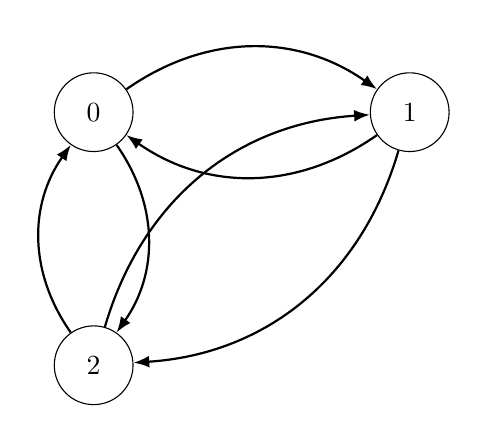
\begin{tikzpicture}[
  state/.style={circle, draw, minimum size=10mm},
  edge/.style={-{Latex[length=2mm]}, thick},
  bend angle=35
]
\node[state] (0) {$0$};
\node[state, right=30mm of 0] (1) {$1$};
\node[state, below=22mm of 0] (2) {$2$};

\draw[edge] (0) edge[bend left] node[above] {} (1);
\draw[edge] (1) edge[bend left] node[below] {} (0);
\draw[edge] (0) edge[bend left] node[left] {} (2);
\draw[edge] (2) edge[bend left] node[right] {} (0);
\draw[edge] (1) edge[bend left] node[right] {} (2);
\draw[edge] (2) edge[bend left] node[left] {} (1);
\end{tikzpicture}
\end{center}

Is the chain irreducible?
\end{example}

\begin{answer}
Yes. From every state, we can reach every other state:
\[
0\leftrightarrow 1,\qquad 0\leftrightarrow 2,\qquad 1\leftrightarrow 2.
\]
Therefore all states communicate with each other.

Hence the chain is irreducible.
\[
\boxed{\text{Irreducible}}
\]
\end{answer}

\begin{example}[Reducible Chain with an Absorbing State]
Consider the transition diagram:

\begin{center}
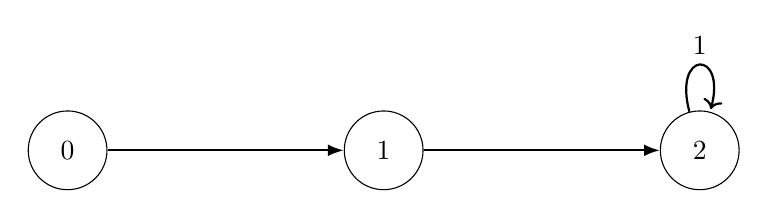
\begin{tikzpicture}[
  state/.style={circle, draw, minimum size=10mm},
  edge/.style={-{Latex[length=2mm]}, thick},
  bend angle=35
]
\node[state] (0) {$0$};
\node[state, right=30mm of 0] (1) {$1$};
\node[state, right=30mm of 1] (2) {$2$};

\draw[edge] (0) -- node[above] {} (1);
\draw[edge] (1) -- node[above] {} (2);
\draw[edge] (2) edge[loop above] node {$1$} (2);
\end{tikzpicture}
\end{center}

Is the chain irreducible?
\end{example}

\begin{answer}
No. We have
\[
0\to 1,\qquad 1\to 2.
\]
But from state $2$, the chain cannot go back to state $1$ or state $0$ because state $2$ is absorbing.

So state $0$ and state $2$ do not communicate.

Therefore the chain is not irreducible.
\[
\boxed{\text{Reducible}}
\]
\end{answer}

\begin{example}[Matrix Example]
Consider
\[
P=
\begin{pmatrix}
0.5 & 0.5 & 0\\
0.2 & 0.3 & 0.5\\
0.1 & 0 & 0.9
\end{pmatrix}.
\]
Is the chain irreducible?
\end{example}

\begin{answer}
The positive entries show the direct transitions:
\[
0\to 0,\quad 0\to 1,
\]
\[
1\to 0,\quad 1\to 1,\quad 1\to 2,
\]
\[
2\to 0,\quad 2\to 2.
\]

Now check communication:

From state $0$, we can go to state $1$. From state $1$, we can go to state $2$. Therefore
\[
0\to 2.
\]

From state $2$, we can go to state $0$. Therefore
\[
2\to 0.
\]

Also, from state $2$, we can go to state $0$, then to state $1$. Therefore
\[
2\to 1.
\]

Every state can reach every other state. Hence the chain is irreducible.
\[
\boxed{\text{Irreducible}}
\]
\end{answer}

\section{Practice Questions}

\begin{enumerate}[label=\textbf{Q\arabic*.}, leftmargin=1.2cm]
    \item Consider the transition diagram:

    \begin{center}
    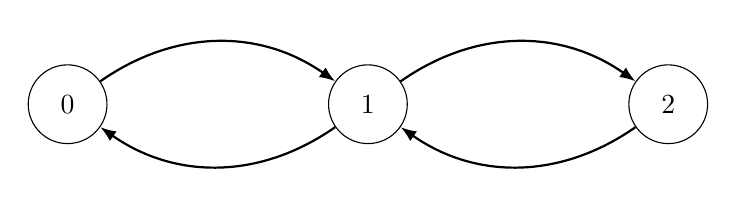
\begin{tikzpicture}[
      state/.style={circle, draw, minimum size=10mm},
      edge/.style={-{Latex[length=2mm]}, thick},
      bend angle=35
    ]
    \node[state] (0) {$0$};
    \node[state, right=28mm of 0] (1) {$1$};
    \node[state, right=28mm of 1] (2) {$2$};
    \draw[edge] (0) edge[bend left] (1);
    \draw[edge] (1) edge[bend left] (0);
    \draw[edge] (1) edge[bend left] (2);
    \draw[edge] (2) edge[bend left] (1);
    \end{tikzpicture}
    \end{center}

    Is the chain irreducible?

    \item Consider the transition diagram:

    \begin{center}
    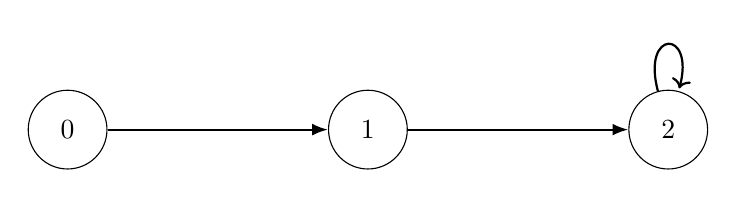
\begin{tikzpicture}[
      state/.style={circle, draw, minimum size=10mm},
      edge/.style={-{Latex[length=2mm]}, thick},
      bend angle=35
    ]
    \node[state] (0) {$0$};
    \node[state, right=28mm of 0] (1) {$1$};
    \node[state, right=28mm of 1] (2) {$2$};
    \draw[edge] (0) -- (1);
    \draw[edge] (1) -- (2);
    \draw[edge] (2) edge[loop above] (2);
    \end{tikzpicture}
    \end{center}

    Is the chain irreducible?

    \item Consider the transition diagram:

    \begin{center}
    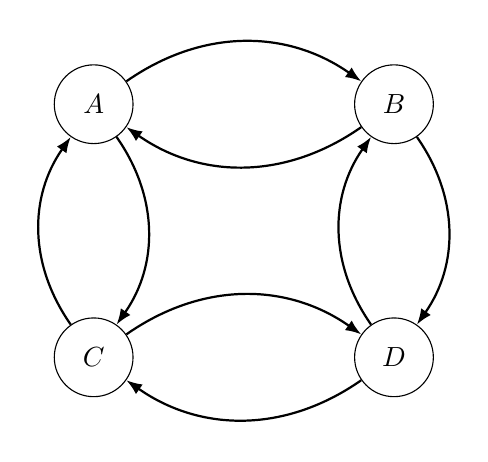
\begin{tikzpicture}[
      state/.style={circle, draw, minimum size=10mm},
      edge/.style={-{Latex[length=2mm]}, thick},
      bend angle=35
    ]
    \node[state] (A) {$A$};
    \node[state, right=28mm of A] (B) {$B$};
    \node[state, below=22mm of A] (C) {$C$};
    \node[state, below=22mm of B] (D) {$D$};
    \draw[edge] (A) edge[bend left] (B);
    \draw[edge] (B) edge[bend left] (A);
    \draw[edge] (B) edge[bend left] (D);
    \draw[edge] (D) edge[bend left] (B);
    \draw[edge] (A) edge[bend left] (C);
    \draw[edge] (C) edge[bend left] (A);
    \draw[edge] (C) edge[bend left] (D);
    \draw[edge] (D) edge[bend left] (C);
    \end{tikzpicture}
    \end{center}

    Is the chain irreducible?

    \item Consider
    \[
    P=
    \begin{pmatrix}
    0.5 & 0.5 & 0\\
    0.5 & 0.5 & 0\\
    0.2 & 0.3 & 0.5
    \end{pmatrix}.
    \]
    Is the chain irreducible?

    \item Consider
    \[
    P=
    \begin{pmatrix}
    0.2 & 0.8 & 0\\
    0 & 0.3 & 0.7\\
    0.6 & 0 & 0.4
    \end{pmatrix}.
    \]
    Is the chain irreducible?

    \item Consider
    \[
    P=
    \begin{pmatrix}
    1 & 0 & 0\\
    0.4 & 0.2 & 0.4\\
    0 & 0 & 1
    \end{pmatrix}.
    \]
    Is the chain irreducible?

    \item A Markov chain has communicating classes
    \[
    \{0,1\},\qquad \{2,3,4\}.
    \]
    Is the chain irreducible?

    \item A Markov chain has state space
    \[
    S=\{0,1,2,3\}.
    \]
    From every state, it is possible to reach state $0$, and from state $0$, it is possible to reach every state. Is the chain irreducible?
\end{enumerate}

\section{Answers}

\subsection*{Answer 1}

The diagram has two-way movement between $0$ and $1$, and two-way movement between $1$ and $2$:
\[
0\leftrightarrow 1,
\qquad
1\leftrightarrow 2.
\]

Also, $0$ can reach $2$ through $1$:
\[
0\to 1\to 2.
\]
Similarly, $2$ can reach $0$ through $1$:
\[
2\to 1\to 0.
\]

Thus every state can reach every other state.

\[
\boxed{\text{Irreducible}}
\]

\subsection*{Answer 2}

The chain has paths
\[
0\to 1\to 2.
\]
But state $2$ has only a self-loop, so from state $2$ we cannot return to state $1$ or state $0$.

Therefore not all states communicate.

\[
\boxed{\text{Reducible}}
\]

\subsection*{Answer 3}

The diagram is one connected two-way system. From each state, we can move to neighbouring states and eventually reach all other states.

For example:
\[
A\to B\to D,
\]
\[
D\to C\to A,
\]
\[
B\to A\to C.
\]

Every state can reach every other state.

\[
\boxed{\text{Irreducible}}
\]

\subsection*{Answer 4}

The transition matrix is
\[
P=
\begin{pmatrix}
0.5 & 0.5 & 0\\
0.5 & 0.5 & 0\\
0.2 & 0.3 & 0.5
\end{pmatrix}.
\]

States $0$ and $1$ communicate with each other:
\[
0\leftrightarrow 1.
\]

From state $2$, we can go to states $0$ and $1$. However, from states $0$ and $1$, there is no path to state $2$, because
\[
p_{02}=0,\qquad p_{12}=0.
\]

Therefore state $2$ does not communicate with states $0$ and $1$.

\[
\boxed{\text{Reducible}}
\]

\subsection*{Answer 5}

The positive direct transitions are:
\[
0\to 0,\quad 0\to 1,
\]
\[
1\to 1,\quad 1\to 2,
\]
\[
2\to 0,\quad 2\to 2.
\]

Now check reachability:

From $0$:
\[
0\to 1\to 2.
\]

From $1$:
\[
1\to 2\to 0.
\]

From $2$:
\[
2\to 0\to 1.
\]

Thus every state can reach every other state.

\[
\boxed{\text{Irreducible}}
\]

\subsection*{Answer 6}

The transition matrix is
\[
P=
\begin{pmatrix}
1 & 0 & 0\\
0.4 & 0.2 & 0.4\\
0 & 0 & 1
\end{pmatrix}.
\]

State $0$ is absorbing because
\[
p_{00}=1.
\]
State $2$ is also absorbing because
\[
p_{22}=1.
\]

From state $1$, we can go to state $0$ or state $2$. But once we enter state $0$, we cannot leave it. Once we enter state $2$, we cannot leave it.

So state $0$ and state $2$ do not communicate with state $1$, and they do not communicate with each other.

\[
\boxed{\text{Reducible}}
\]

\subsection*{Answer 7}

The chain has two communicating classes:
\[
\{0,1\}
\quad\text{and}\quad
\{2,3,4\}.
\]

For a chain to be irreducible, the whole state space must be one communicating class.

Since there is more than one communicating class, the chain is not irreducible.

\[
\boxed{\text{Reducible}}
\]

\subsection*{Answer 8}

We are told:
\begin{itemize}[leftmargin=1.2cm]
    \item from every state, it is possible to reach state $0$,
    \item from state $0$, it is possible to reach every state.
\end{itemize}

Take any two states $i$ and $j$. Since $i$ can reach state $0$,
\[
i\to 0.
\]
Since state $0$ can reach $j$,
\[
0\to j.
\]
Therefore,
\[
i\to 0\to j.
\]
So every state $i$ can reach every state $j$.

Also, by the same argument, $j$ can reach $i$.

Hence every pair of states communicates, and the chain is irreducible.

\[
\boxed{\text{Irreducible}}
\]

\end{document}
